\documentclass[a4paper,10pt]{jsarticle}
\usepackage{amsmath}
\usepackage{bm}
\usepackage[dvipdfmx]{graphicx}
\usepackage[dvipdfmx]{hyperref}
\usepackage{pxjahyper}
\usepackage{url}
\setlength{\textwidth}{165mm}
\setlength{\marginparwidth}{40mm}
\setlength{\textheight}{225mm}
\setlength{\topmargin}{-5mm}
\setlength{\oddsidemargin}{-3.5mm}
\def\vector#1{\mbox{\boldmath $#1$}}
\newcommand{\AmSLaTeX}{
$\mathcal A$\lower.4ex\hbox{$\!\mathcal M\!$}$\mathcal S$-\LaTeX}
\newcommand{\PS}{{\scshape Post\-Script}}
\def\BibTeX{{\rmfamily B\kern-.05em{\scshape i\kern-.025em b}\kern-.08em
 T\kern-.1667em\lower.7ex\hbox{E}\kern-.125em X}}
\newcommand{\pderiv}[2]{{\partial#1\over\partial#2}}
\newcommand{\deriv}[2]{{{\rm d}#1\over{\rm d}#2}}
\newcommand{\dderiv}[2]{{{\rm d}^2#1\over{\rm d}#2^2}}
\newcommand{\DeLta}{{\mit\Delta}}
\renewcommand{\d}{{\rm d}}
\def\wcaption#1{\caption[]{\parbox[t]{100mm}{#1}}}
\def\rm#1{\mathrm{#1}}
\def\tempC{^\circ \rm{C}}
\makeatletter
\def\subsection{\@startsection {subsection}{1}{\z@}{-3.5ex plus -1ex minus-.2ex}{2.3ex plus .2ex}{\normalsize\bf}}
\makeatother
\makeatletter
%\def\section{\@startsection {section}{1}{\z@}{-3.5ex plus -1ex minus % -.2ex}{2.3ex plus .2ex}{\Large\bf}}
\def\section{\@startsection {section}{1}{\z@}{-3.5ex plus -1ex minus-.2ex}{2.3ex plus .2ex}{\normalsize\bf}}
\makeatother
\makeatletter
\def\@seccntformat#1{\@ifundefined{#1@cntformat}%
{\csname the#1\endcsname\quad}%      default
{\csname #1@cntformat\endcsname}%    enable individual control}
}
\makeatother
%%%%%%%%%%%%%%%%%%%%%%%%%%%%%%%%%%%%%%%%%%%%%%%%%%%%%%%%%%%%%%%%%%%%%%
\begin{document}

\begin{center}
  {\Large{\bf DockerとRos2 によるシミュレーション環境の構築}} \\
\end{center}

%%%%%%%%%%%%%%%%%%%%%%%%%%%%%%%%%%%%%%%%%%%%%%%%%%%%%%%%%%%%%%%%%%%%%%
\section{これだけ知ってればまず動く!}
PCに環境が出来あがった状態であることが前提のセクションです。まだ作ってない人は、\ref{making environment}とりあえず環境作ろう を先に見てください\\
\subsection{フローチャート}
windows(またはMac上で)\\
docker start hr\_education (またはdocker start hr\_arm\_robot\_simenv)\\\\
ウェブブラウザで次を検索\\
http://127.0.0.1:6080\\\\
ウェブ上のlinux環境でTerminatorを起動。Terminator上で次を実行\\
ros2 launch angle\_control angle\_control\_gazebo\_included.launch.py\\\\
シミュレーション環境が現れます。\\
続いて別のTerminatorを起動して、目的のフォルダに移動\\
cd \verb|~|/hr\_ws/src/crane\_x7\_hr\_edu/move\_robot/examples/ (自分のコードの場合はexamples を motions に変更)\\\\
フォルダー下で用意したコードを実行します\\
python3 your\_code\_name.py (you\_code\_nameは自分のコードの名前に変更)\\\\
自分のコードを編集したかったら次のコードでVScodiumを開きましょう\\
codium .\\\\
終わったら必ずコンテナを必ず止めましょう。windows(またはMac上で)\\
docker stop hr\_education(またはdocker stop hr\_arm\_robot\_simenv)

\subsection{環境の立ち上げ方(詳しく)}
環境はdockerでできているので、まずはコンテナを起動しましょう。起動する前に対象の名前を確認しておきます。windows powershell またはターミナルを開いて、\\
\begin{center}
docker ps -a\\
\end{center}
を実行してください。多分図\ref{dockerps}のような表示が出ると思います(皆さんのPCだと上の一つだけかもしれないですが問題ありません)。
\begin{figure}[ht]
  \begin{center}
    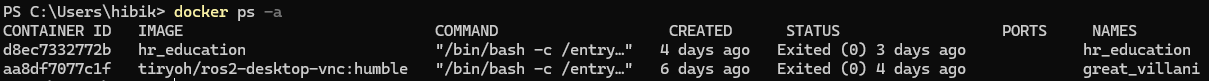
\includegraphics[width=16cm]{pictures/docker_ps_a.png}
    \caption{docker ps}
    \label{dockerps}
  \end{center}
\end{figure}
IMAGEタグの下がhr\_education, またはhr\_arm\_robot\_simenvとなっているのが、前回作ったDocker Containerです。
目的のコンテナが見つかったら、NAMESのところを確認してください。この場合hr\_educationが使用するものです。\\
さて、コンテナをスタートさせるために次のコマンドを入力してください。\\
\begin{center}
docekr start hr\_education
\end{center}
図\ref{dockerstart}のように表示されればokです。\\
\begin{figure}[ht]
  \begin{center}
    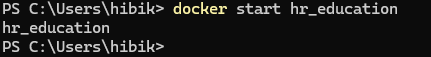
\includegraphics[width=8cm]{pictures/docker_start_container.png}
    \caption{docker start your\_container\_name}
    \label{dockerstart}
  \end{center}
\end{figure}

では、このコンテナのデスクトップ画面に行ってみましょう。ウェブブラウザを開いて、
\begin{center}
  http://127.0.0.1:6080
\end{center}
を検索してください。\\
\begin{figure}[ht]
  \begin{center}
    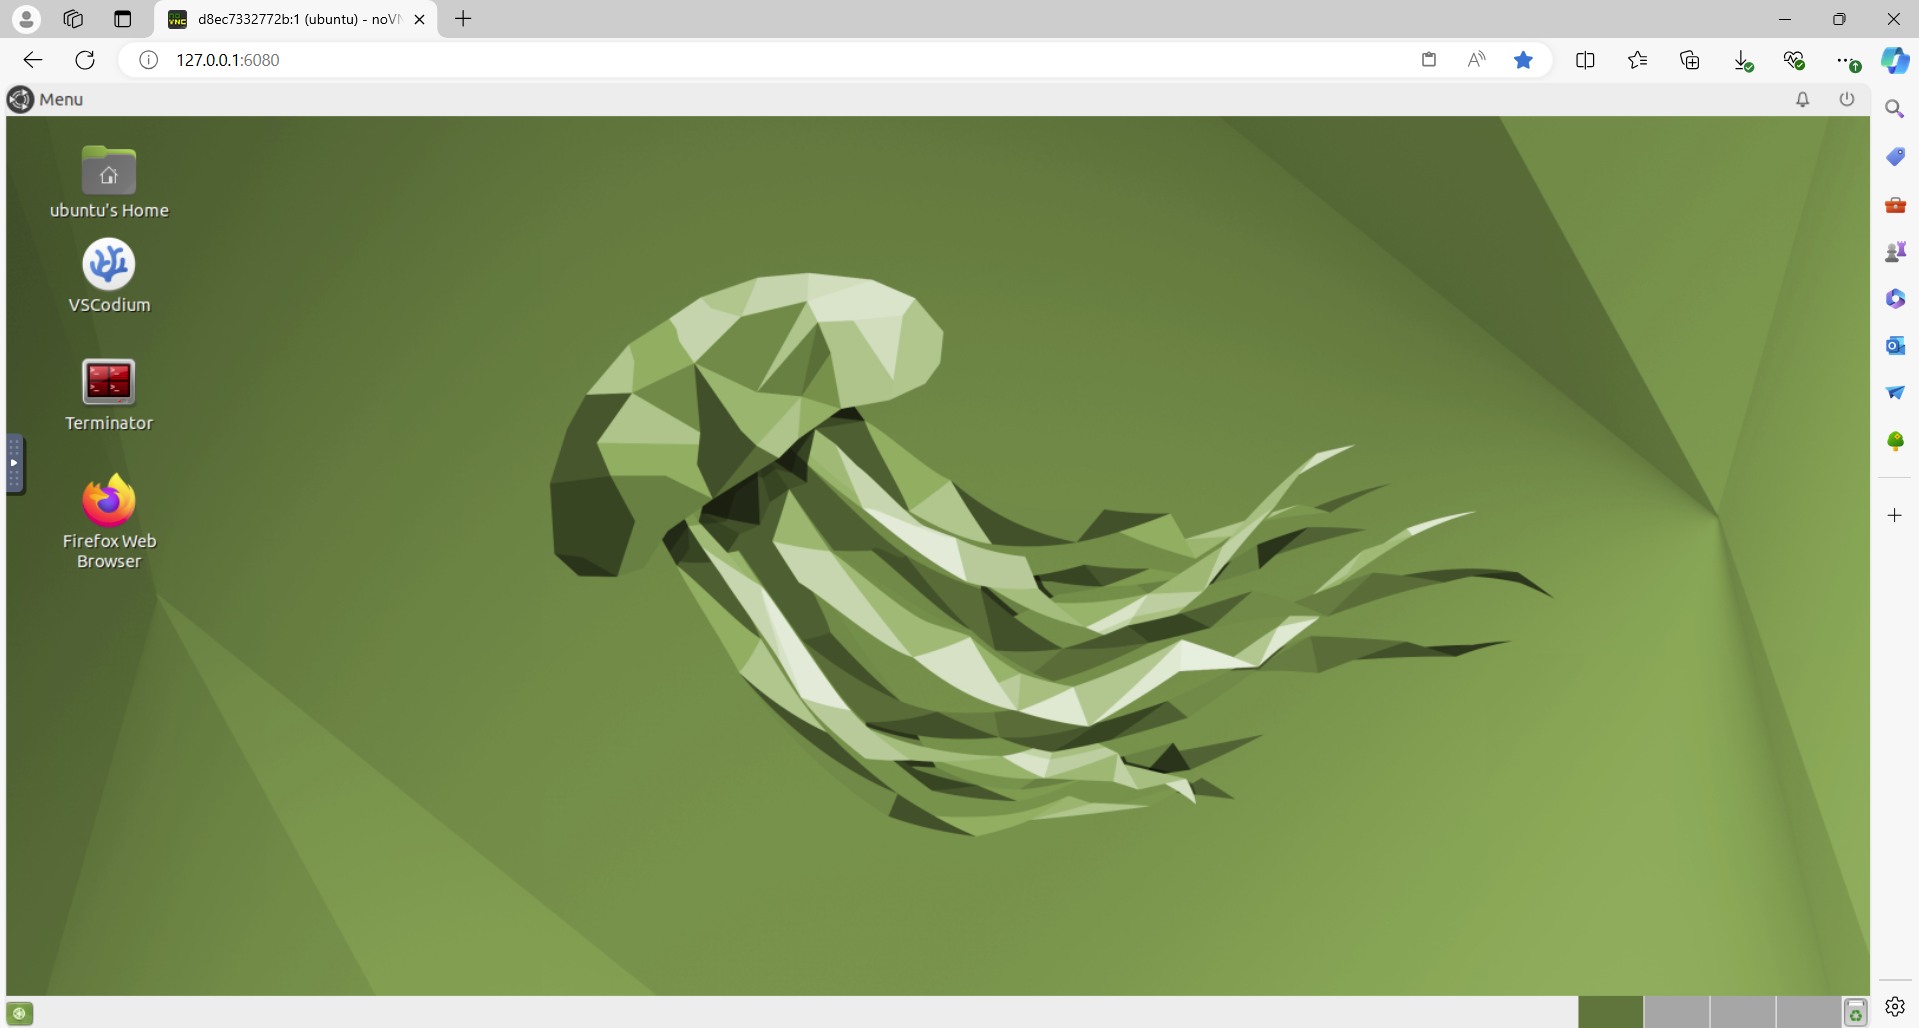
\includegraphics[width=8cm]{pictures/webbrouser.png}
    \caption{ubuntu desktop}
    \label{ubuntudesktop}
  \end{center}
\end{figure}

図\ref{ubuntudesktop}のようになればokです。
これから先はこのブラウザ上のデスクトップで作業を進めていきます。基本的にコマンドはTerminatorというところに打ち込んでいきます。\\
ではまず、用意してあるアームロボットのシミュレーションを立ち上げてみましょう。Terminatorを開いて
\begin{center}
  ros2 launch angle\_control angle\_control\_gazebo\_included.launch.py
  \label{launchcode}
\end{center}
を実行しましょう(図\ref{launch})\\
\begin{figure}[ht]
  \begin{center}
    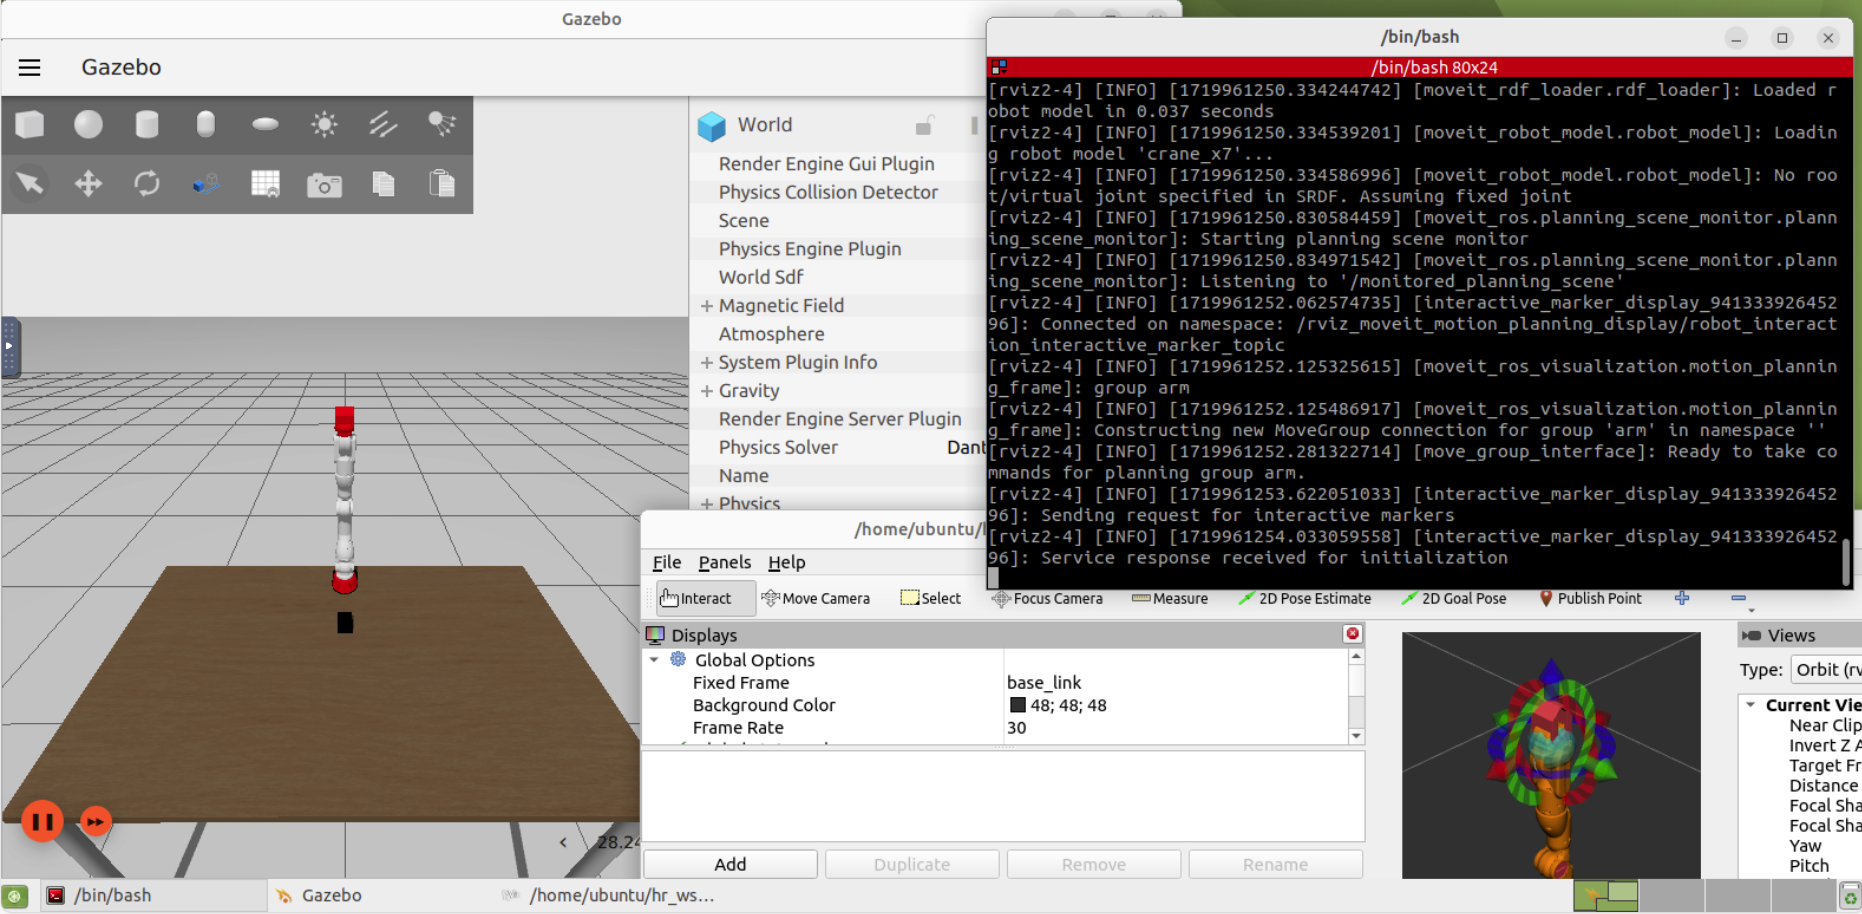
\includegraphics[width=12cm]{pictures/launch.png}
    \caption{simulator}
    \label{launch}
  \end{center}
\end{figure}

初回は時間がかかります。また、ウェブ上で動かしているのでバグることも多いので、うまくいってなさそうだったらctlr+Cで一旦停止し、もう一度実行してください。\\
では、プログラムのコードがあるところに行きましょう。新しいTerminatorを開き、次のコマンドで目的の場所まで行きます。
\begin{center}
  cd \verb|~|/hr\_ws/src/crane\_x7\_hr\_edu/move\_robot/examples/
\end{center}
ではコードを実行してみましょう。
\begin{center}
  python your\_code\_name.py
\end{center}
your\_code\_nameは実行したいコードの名前に置き換えてください。今回はあらかじめ用意してあるwave.pyを使用しています。
\begin{figure}[ht]
  \begin{center}
    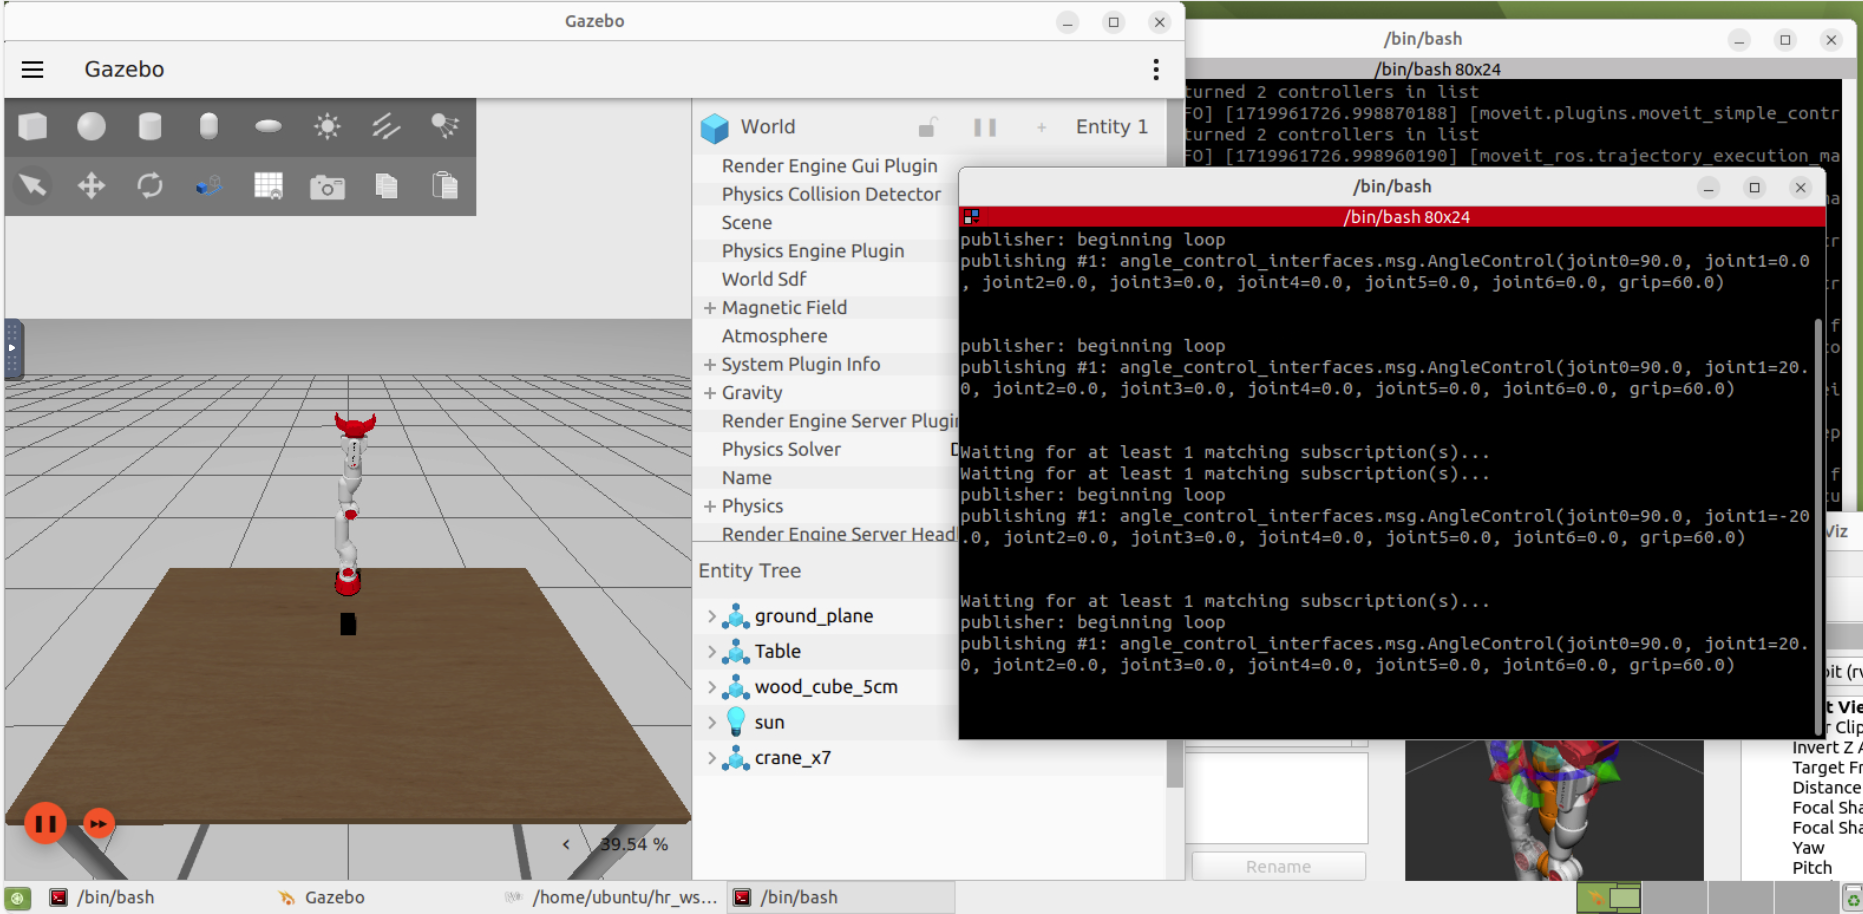
\includegraphics[width=12cm]{pictures/wave.png}
    \caption{move robot}
    \label{moverobot}
  \end{center}
\end{figure}
図\ref{moverobot}のように2つのTerminatorに謎の文字列が表示されて、ロボットが動き出します。\\
動かなかったらシミュレータを再度動かしてみてください\ref{launchcode}\\
これで環境を立ち上げることができるようになりました!お疲れ様です。

\section{コードの書き方}
さて、コードを書いていきましょう。皆さんのコードはmotionsというところに書いていってもらいます。まずは目的の場所に移動して
\begin{center}
  cd \verb|~|/hr\_ws/src/crane\_x7\_hr\_edu/move\_robot/
\end{center}
VScoduimを起動しましょう図\ref{openvscodium}。\\
\begin{center}
  codium .
\end{center}
\begin{figure}[ht]
  \begin{center}
    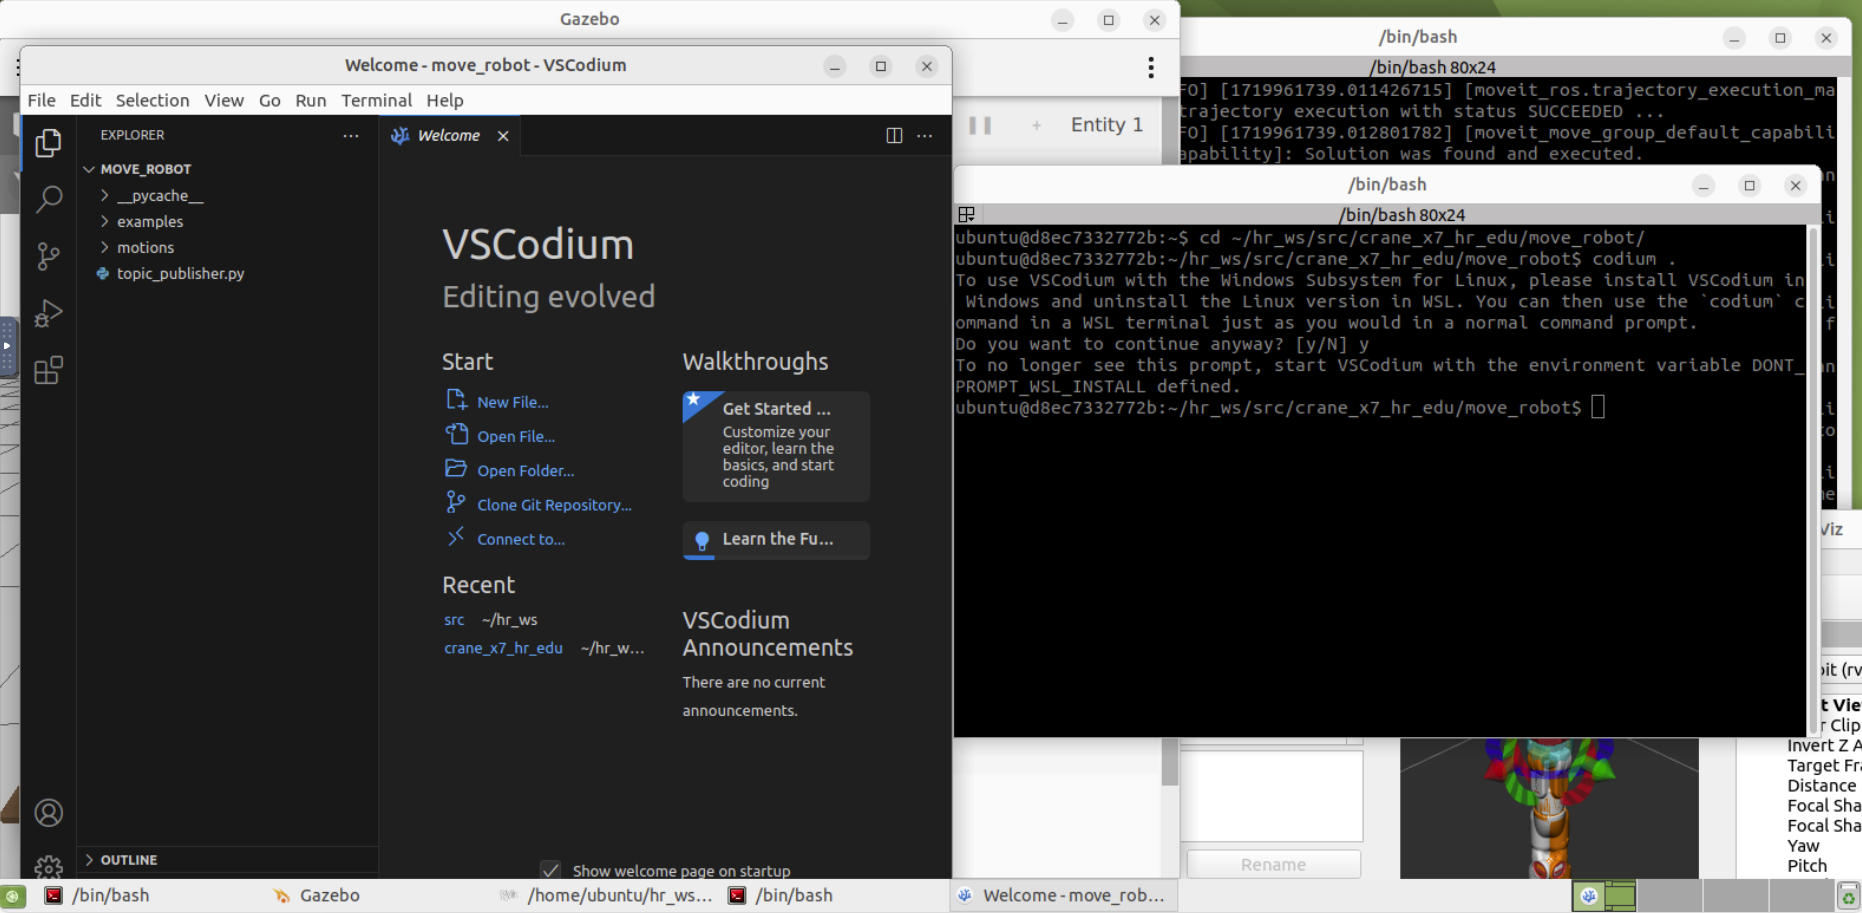
\includegraphics[width=15cm]{pictures/codium.png}
    \caption{open vscodium}
    \label{openvscodium}
  \end{center}
\end{figure}

コードを書きやすいように色々下設定を済ませてあるので、まずは作成した.pyファイルに次の呪文を書き入れてください。
pythonファイルは、motionsフォルダ(なかったら作ってください)直下に入れましょう
\begin{verbatim}
import sys

sys.path.append("..")
from topic_publisher import angle_write

\end{verbatim}
これで関数「angle\_write」が使えるようになります。\\
angle\_write()関数は大きさが8のリストを受け取り、ロボットに角度情報を送るプログラムです。
リストの0から6までが関節角度を、7がハンドの角度を指定します。例としてwave.pyを見てみましょう。
\begin{verbatim}
import sys

sys.path.append("..")
from topic_publisher import angle_write

wave = [
    [90,0,0,0,0,0,0,60],
    [90,20,0,0,0,0,0,60],
    [90,-20,0,0,0,0,0,60],
    [90,20,0,0,0,0,0,60],
    [90,-20,0,0,0,0,0,60],
    [90,0,0,0,0,0,0,60]
]

for value in wave:
    angle_write(value)
\end{verbatim}
wave=...のところで6つの角度を順番に指定した2重リストを作っています。後はfor文で指定した角度を順番に回し、ロボットを動かしています。
ここで、機体の限界を超える角度を入力してもロボットは反応しません。また、指示角度にロボットが動ききるまでは次の命令を受け付けない仕様になっています。


\section{とりあえず環境作ろう}
\label{making environment}
環境を作るため、GitとDockerをダウンロードする必要があります。\\
Macの人はGitとDocker Desktopをそれぞれ調べ、ダウンロードしてください。\\
Windowsの人はpowershellを開いて次のコマンドをそれぞれ打ち込みましょう。
\begin{verbatim}
  winget install Git.Git
  winget insatll Docker.DockerDesktop
\end{verbatim}
かなり時間がかかりますがダウンロードできます。\\
ダウンロードが終わったら、PCを再起動してください。\\
再起動後にもう一度powershellを開き
\begin{verbatim}
  git --version
  docker --version
\end{verbatim}
をそれぞれ実行しましょう。図\ref{version}のような表示が出たらokです。
\begin{figure}[ht]
  \begin{center}
    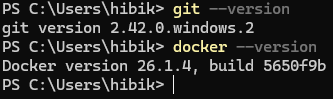
\includegraphics[width=8cm]{pictures/version.png}
    \caption{version information}
    \label{version}
  \end{center}
\end{figure}

それでは、DockerのImageを作成していきましょう。まずはいつもロボメカの作業をしているディレクトリに移動してください。
移動先で次のコマンドを実行します。
\begin{center}
  git clone -b master \verb|https://github.com/rmf-hru-wg/hr_arm_robot_simenv.git|
\end{center}
ディレクトリで
\begin{center}
  ls ./hr\_arm\_robot\_simenv
\end{center}
を実行して図\ref{lscheck}のように表示されたら成功です。
\begin{figure}[ht]
  \begin{center}
    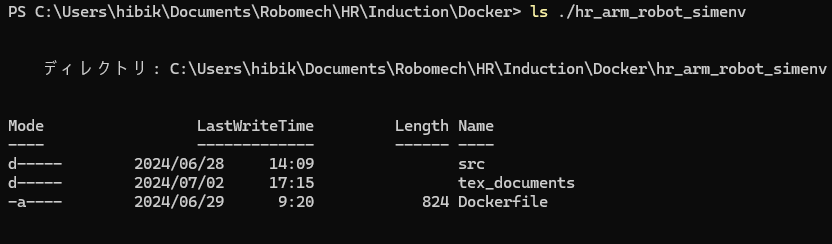
\includegraphics[width=12cm]{pictures/ls_check.png}
    \caption{ls check}
    \label{lscheck}
  \end{center}
\end{figure}

ではImageを作っていきましょう。まずは先ほどcloneしたディレクトリに移動して
\begin{center}
  cd hr\_arm\_robot\_simenv
\end{center}
imageを作ります。
\begin{center}
  docker image build -t hr\_arm\_robot\_simenv .
\end{center}
\begin{figure}[ht]
  \begin{center}
    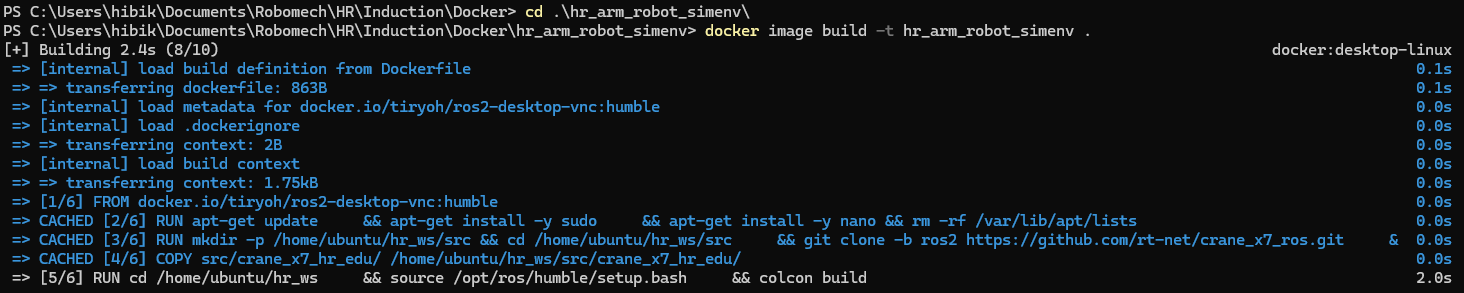
\includegraphics[width=12cm]{pictures/build_image.png}
    \caption{build image}
    \label{buildimage}
  \end{center}
\end{figure}

図\ref{buildimage}のように青い行がたくさん表示されたら成功です。30分くらいかかるので気長に待ちましょう。
なんかうまくいかなかった場合は\ref{trouble}トラブルシューティング へ\\

では作成したイメージを確認しましょう
\begin{center}
  docker images
\end{center}
図\ref{images}のように表示されたらokです。皆さんの場合はREPOSITORYの下の名前がhr\_educationではなく、hr\_arm\_robot\_simenvとなるはずです。
\begin{figure}[ht]
  \begin{center}
    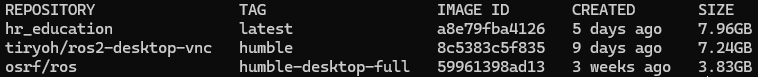
\includegraphics[width=12cm]{pictures/images.png}
    \caption{images}
    \label{images}
  \end{center}
\end{figure}

ではこのimageを実際に使えるようにしてみましょう。
\begin{center}
  docker run -p 6080:80 --name hr\_education hr\_arm\_robot\_simenv
\end{center}
大体図\ref{dockerrun}のようなものが表示されればokです。
\begin{figure}[ht]
  \begin{center}
    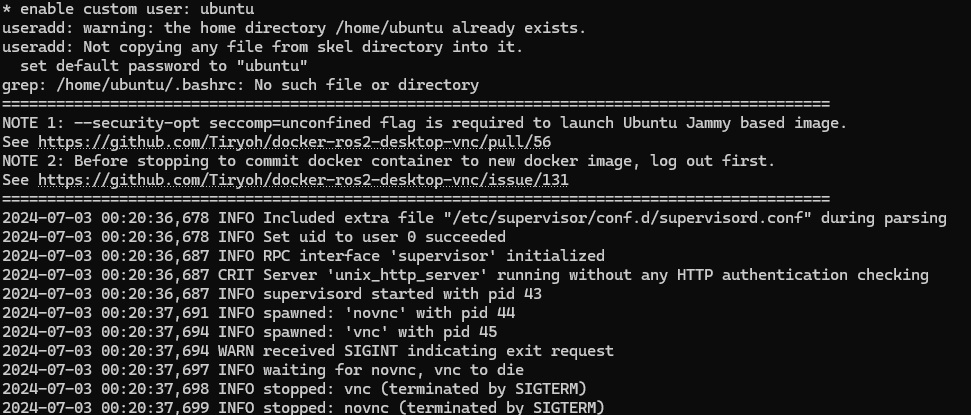
\includegraphics[width=8cm]{pictures/docker_run.png}
    \caption{docker run}
    \label{dockerrun}
  \end{center}
\end{figure}

これでcontainerが動き出しました。確認してみましょう。ほかのshellを開いて、
\begin{center}
  docker ps
\end{center}
図\ref{dockerps}のように表示されていればokです。大事なのはNAMESのところで、ここがhr\_educationなら大丈夫です。
\begin{figure}[ht]
  \begin{center}
    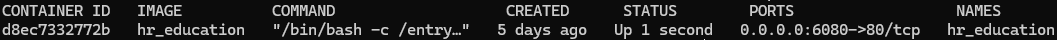
\includegraphics[width=16cm]{pictures/docker_ps.png}
    \caption{docker ps}
    \label{dockerps}
  \end{center}
\end{figure}

使い終わったら必ず
\begin{center}
  docker stop hr\_education
\end{center}
で動作を止めましょう。PCに悪いです。\\
次にコンテナを再起動したいときは
\begin{center}
  docekr start hr\_education
\end{center}
で始めることができます。ではコンテナを再度起動して(docker start hr\_education)デスクトップに接続しましょう。ブラウザで
\begin{center}
  http://127.0.0.1:6080
\end{center}
を検索してください。開けたらTerminatorを起動しましょう。開けたら、
\begin{center}
  \verb|echo 'source /home/ubuntu/hr_ws/install/local_setup.bash' >> ~/.bashrc|
\end{center}
と打ち込んでください(図\ref{echo})。
\begin{figure}[ht]
  \begin{center}
    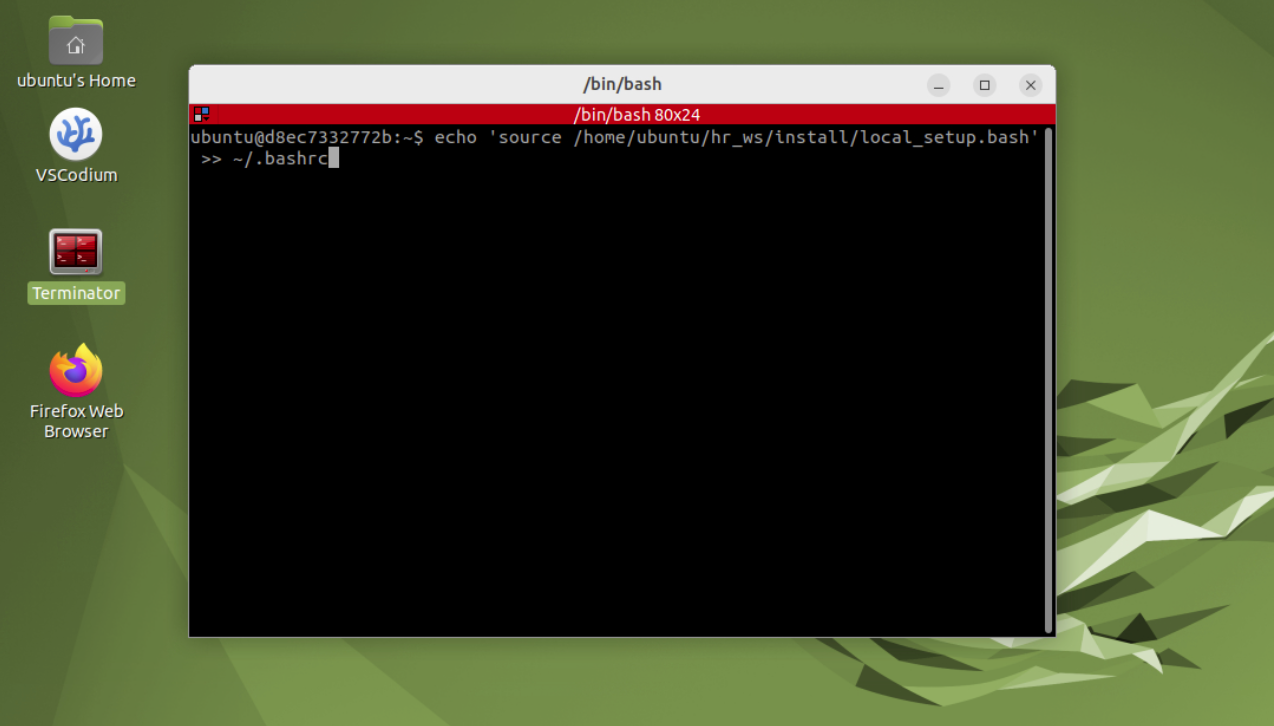
\includegraphics[width=12cm]{pictures/echo.png}
    \caption{echo}
    \label{echo}
  \end{center}
\end{figure}

Terminatorを再起動したら環境完成です。

\section{Dockerとは}
後で書きます。
\section{Rosとは}
後で書きます。
\section{書いてあるコードの説明}
後で書きます。
\section{これらを使うと何ができるか?}
後で書きます。
\section{トラブルシューティング}
\label{trouble}
\subsection{ありそうなミス}
ubuntuのデスクトップ(127.0.0.1:6080)では貼り付けのコマンドは Ctrl+Shift+V、コピーは Ctrl+Shift+C。\\
\verb|~|を書き忘れている。\\
echo ....コマンドを打った後にTerminatorを再起動してない\\
python3 じゃなくてpythonって打ってる\\
python3 を実行するディレクトリが違う(exampleまたはmotionsじゃないと動かない)\\


\subsection{docker image build でDockerfile not foundと言われた}
git clone が間違っている可能性があります。一度hr\_arm\_robot\_simenvフォルダを削除し、再度\\
git clone -b master https://....\\
を実行しましょう。-b master を忘れないようにしましょう

\subsection{docker image build が colcon build のところで止まる}
PCのスペックが足りてない可能性があります。Dockerfileを次のように編集してください。
\begin{verbatim}
FROM tiryoh/ros2-desktop-vnc:humble

RUN apt-get update \
    && apt-get install -y sudo \
    && apt-get install -y nano && rm -rf /var/lib/apt/lists

RUN mkdir -p /home/ubuntu/hr_ws/src && cd /home/ubuntu/hr_ws/src \
    # Download crane_x7 repositories
    && git clone -b ros2 https://github.com/rt-net/crane_x7_ros.git \
    && git clone -b ros2 https://github.com/rt-net/crane_x7_description.git\
    # Install dependencies
    && rosdep -y update && apt-get update \
    && rosdep install -r -y -i --from-paths .

# copy some source files
COPY src/crane_x7_hr_edu/ /home/ubuntu/hr_ws/src/crane_x7_hr_edu/

# build all the file
RUN cd /home/ubuntu/hr_ws \
    && source /opt/ros/humble/setup.bash \
    && colcon build --packages-skip angle_conntrol \
    && colcon build --packages-select angle_control

RUN echo 'source /home/ubuntu/hr_ws/install/local_setup.bash' >> ~/.bashrc

\end{verbatim}


\end{document}